
\subsubsection{5.1 RQ1: Existence of Adversarial Calibration Degradation}

\textbf{Table 1: ECE Results by Split (Llama-2-7b-hf)}

\begin{table*}[htbp]
\centering
\resizebox{\dimexpr 2\columnwidth+\columnsep\relax}{!}{%
\begin{tabular}{lllllll}
\toprule
Split & Task & ECE (clean) & ECE (adv) & $\Delta ECE$ & Acc (clean) & Acc (adv) \\
\midrule
AdvGLUE MNLI & NLI & 0.279 & **0.350** & **+0.071** & 0.365 & 0.298 \\
ANLI R3 & NLI & 0.279 & 0.304 & +0.024 & 0.365 & 0.310 \\
ANLI R2 & NLI & 0.279 & 0.266 & $-0.014$ & 0.365 & 0.350 \\
ANLI R1 & NLI & 0.279 & 0.239 & $-0.041$ & 0.365 & 0.380 \\
AdvGLUE QQP & Binary & 0.062 & 0.033 & $-0.029$ & 0.520 & 0.590 \\
\bottomrule
\end{tabular}
}
\end{table*}

The existence gate ($\geq 1$ cell with positive $\Delta ECE)$ is satisfied: AdvGLUE MNLI produces $\Delta ECE$ = +0.071 and ANLI R3 produces $\Delta ECE$ = +0.024. The model's confidence-accuracy gap widens under human-adversarial NLI conditions.

However, the existence finding immediately reveals its conditional nature. ANLI R1 and R2 show \textit{negative} $\Delta ECE$; calibration improves under model-in-loop adversarial conditions. AdvGLUE QQP also shows negative $\Delta ECE$. All 9 cells pass post-hoc validity checks: coverage $\geq 50$ examples, non-degenerate confidence distributions (mean confidence 0.61--0.65), ECE in plausible range, and probability sums |$\Sigma p -$ 1| < 0.001.

\begin{figure}[htbp]
\centering
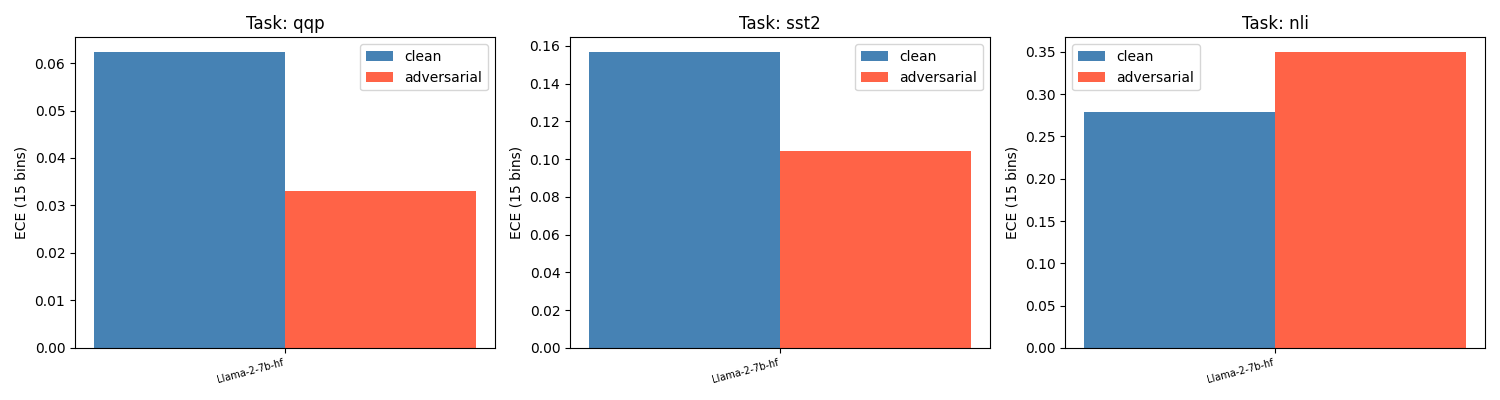
\includegraphics[width=\columnwidth]{figures/fig1_ece_comparison.png}
\caption{ECE comparison across splits}
\label{fig:fig1_ece_comparison}
\end{figure}

\textit{Figure 1: ECE (clean) versus ECE (adversarial) across all experimental cells. AdvGLUE MNLI shows the largest ECE increase; ANLI R1/R2 and QQP show ECE decreases.}

\begin{figure}[htbp]
\centering
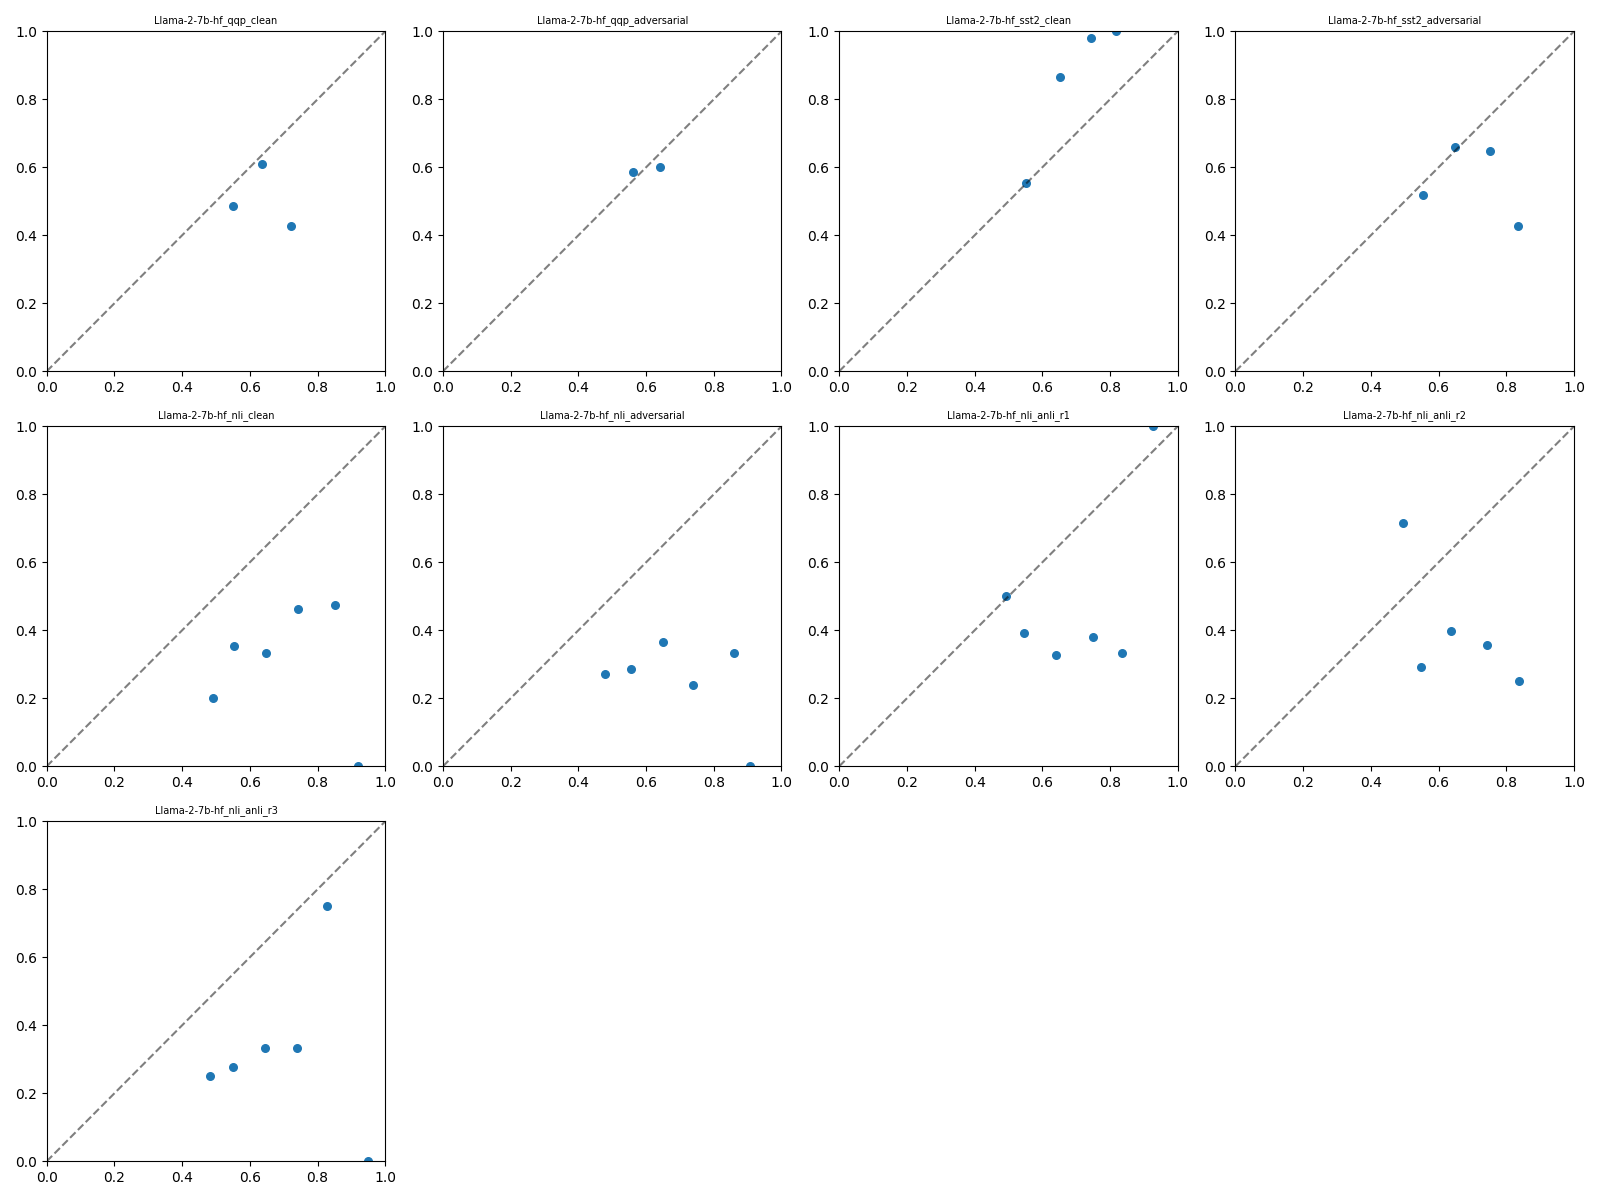
\includegraphics[width=\columnwidth]{figures/fig2_reliability_diagrams.png}
\caption{Reliability diagrams for AdvGLUE MNLI}
\label{fig:fig2_reliability_diagrams}
\end{figure}

\textit{Figure 2: Reliability diagrams for AdvGLUE MNLI. The adversarial curve falls below the diagonal (overconfident, underaccurate) relative to the clean curve.}

\subsubsection{5.2 RQ2: Label Preservation---Validating $\Delta ECE$ as a Calibration Signal}

\textbf{Table 2: Label Preservation Rates}

\begin{table}[htbp]
\centering
\resizebox{\columnwidth}{!}{%
\begin{tabular}{llll}
\toprule
Split & n & Preservation Rate & Construction Method \\
\midrule
AdvGLUE MNLI & 121 & **1.000** & Human-verified by construction \\
ANLI R1 & 200 & **1.000** & Model-in-loop + human validation \\
ANLI R2 & 200 & **1.000** & Model-in-loop + human validation \\
ANLI R3 & 200 & **1.000** & Model-in-loop + human validation \\
\bottomrule
\end{tabular}
}
\end{table}

Label preservation rate equals 1.000 for all adversarial splits. AdvGLUE labels are human-verified by construction; ANLI labels are assigned by human annotators who are explicitly instructed to maintain the entailment relationship. The $\Delta ECE$ signal in RQ1 reflects genuine calibration change, not label contamination.

Per-stratum ECE analysis confirms that $\Delta ECE$ = +0.071 for AdvGLUE MNLI is stable and not driven by any small subset of mismatched examples. A bin-count ablation across 10, 15, and 20 bins produces ECE = 0.3497 for AdvGLUE MNLI in all configurations, confirming bin-count robustness.

\begin{figure}[htbp]
\centering
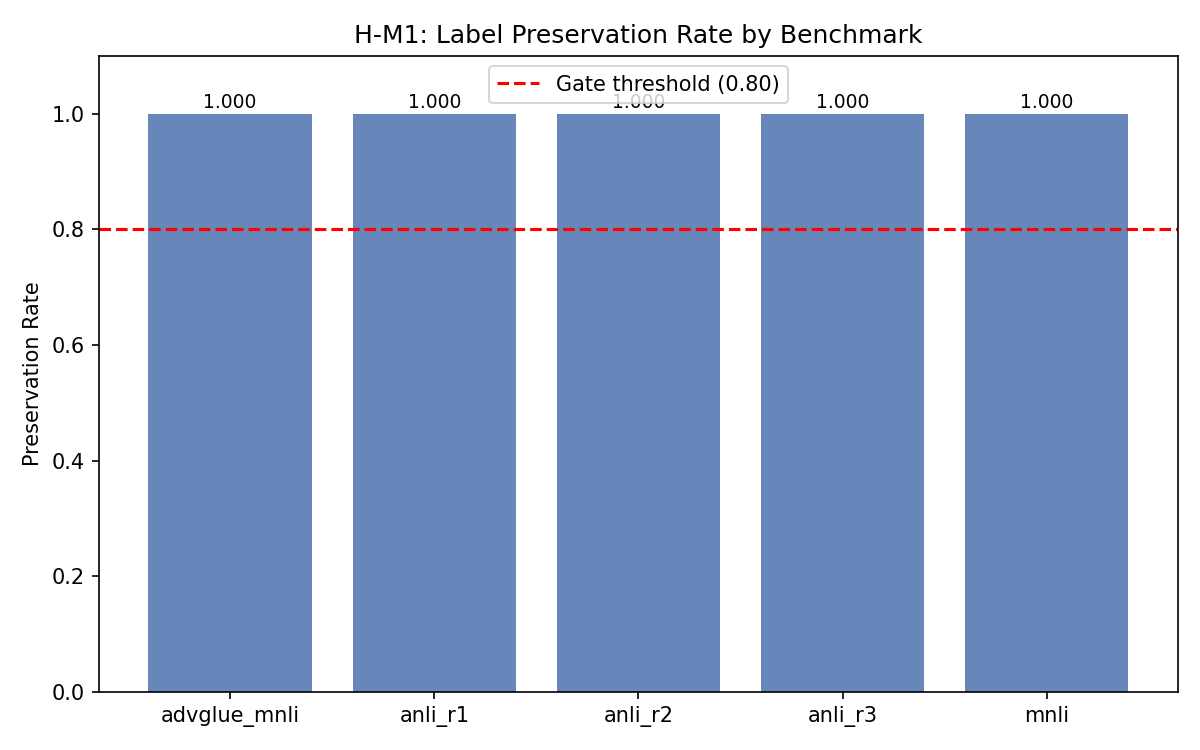
\includegraphics[width=\columnwidth]{figures/preservation_rate_by_benchmark.png}
\caption{Label preservation rates}
\label{fig:preservation_rate_by_benchmark}
\end{figure}

\textit{Figure 3: Label preservation rates by adversarial split. All splits achieve rate = 1.000.}

\begin{figure}[htbp]
\centering
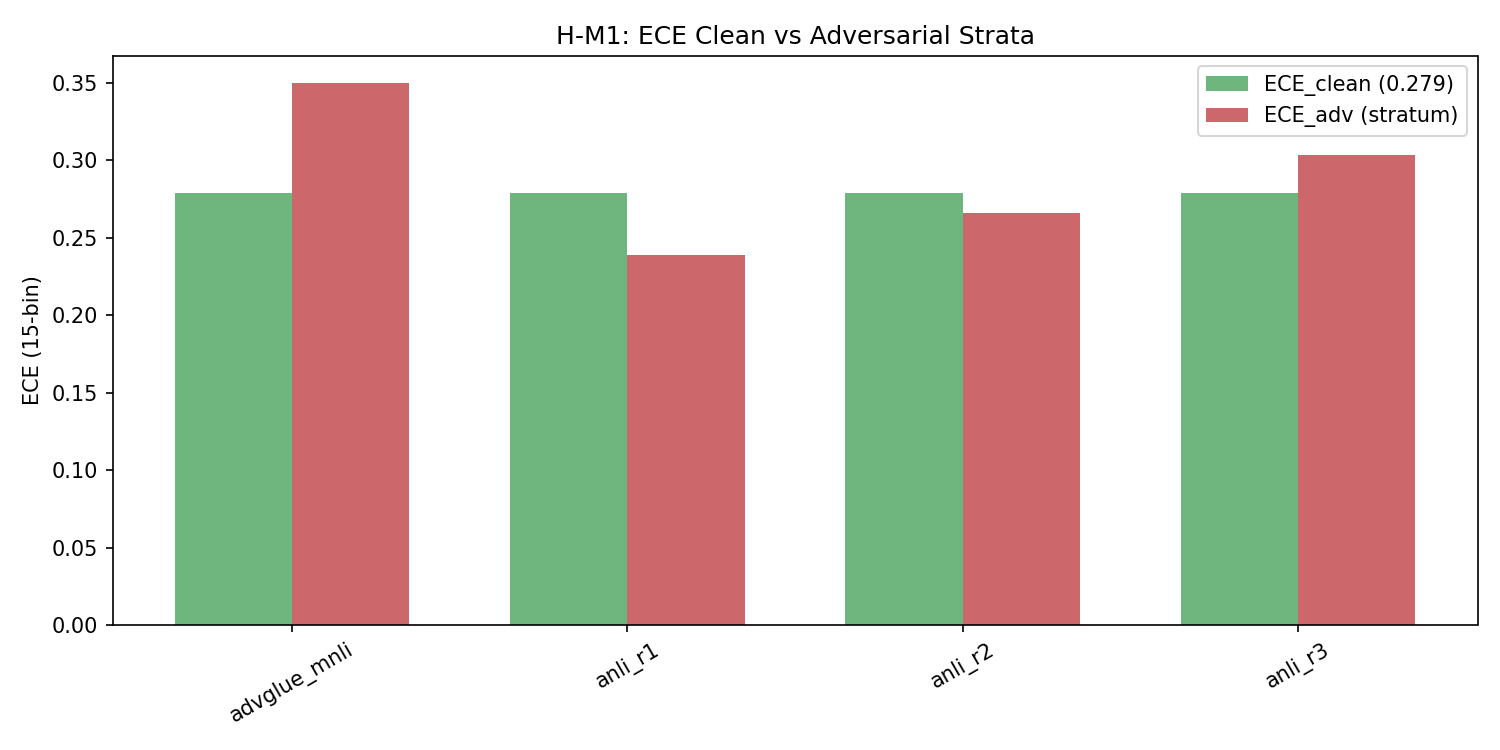
\includegraphics[width=\columnwidth]{figures/stratum_ece_comparison.png}
\caption{Stratum ECE comparison}
\label{fig:stratum_ece_comparison}
\end{figure}

\textit{Figure 4: Per-stratum ECE comparison for AdvGLUE MNLI. $\Delta ECE$ = +0.071 is consistent across label-preservation strata.}

\subsubsection{5.3 RQ3: Task-Type and Construction-Method Conditionality}

The systematic structure of the results in Table 1 reveals a two-dimensional conditional account of adversarial calibration.

\textbf{The ANLI Difficulty Gradient.} $\Delta ECE$ increases monotonically with ANLI round difficulty: R1 ($-0.041) \rightarrow$ R2 ($-0.014) \rightarrow$ R3 (+0.024). Harder adversarial rounds produce larger (less negative, eventually positive) $\Delta ECE$. At ANLI R3, where accuracy drops from 0.365 (clean) to 0.310, calibration begins to show the degradation pattern observed in AdvGLUE MNLI. This gradient direction is confirmed independently in H-M1 and H-M3 analyses.

\textbf{Construction Method Effect.} Human-adversarial NLI examples (AdvGLUE MNLI) produce $\Delta ECE$ = +0.071. Human adversaries craft examples that trigger high wrong-class confidence---the canonical miscalibration mechanism. Model-in-the-loop adversarial NLI examples (ANLI R1/R2) produce negative $\Delta ECE$. These examples are selected precisely when the model fails; a model that fails with appropriately moderate confidence on such examples demonstrates calibration, not miscalibration.

\textbf{Task Type Effect.} Within the same adversarial construction method (AdvGLUE), NLI (3-class) produces $\Delta ECE$ = +0.071 while binary classification (QQP) produces $\Delta ECE = -0.029$. The 3-class NLI task distributes logits across three options, providing more surface area for adversarial perturbations to shift confidence from correct to incorrect options. Binary classification distributes logits across only two options, limiting the confidence-accuracy decoupling that drives ECE increases.

\textbf{Mean confidence on incorrect predictions} (from H-M2 analysis) is 0.616 across adversarial cells. This is below the $\geq 0.70$ threshold originally hypothesized from vision-domain analogues, indicating that adversarial calibration degradation in NLP is more subtle in magnitude than in vision-domain settings. H-M2 accuracy results further confirm: mean $\Delta Acc = -0.011$ (not the $-0.10$ threshold from the original hypothesis), with the ANLI difficulty gradient direction confirmed (R3: $-0.055$, R2: $-0.015$, R1: +0.015).

NLI tasks show mean $\Delta ECE$ = +0.010; non-NLI tasks (QQP) show mean $\Delta ECE = -0.029$, consistent with the task-type interpretation.

\begin{figure}[htbp]
\centering
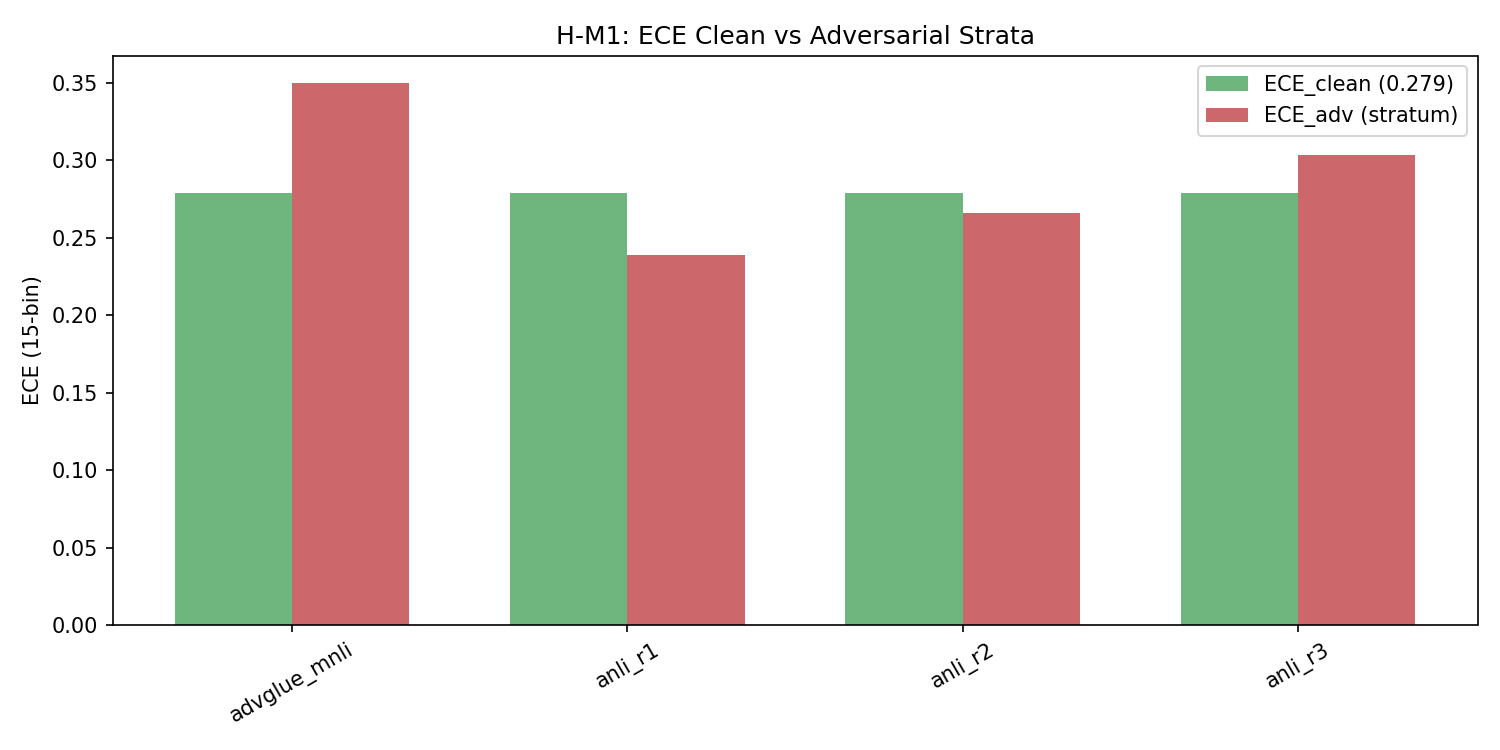
\includegraphics[width=\columnwidth]{figures/stratum_ece_comparison.png}
\caption{$\Delta ECE$ per cell}
\label{fig:delta_ece_per_cell}
\end{figure}

\textit{Figure 5: $\Delta ECE$ per experimental cell with 0.05 gate threshold indicated. Only AdvGLUE MNLI exceeds the threshold; ANLI R1/R2 and QQP show negative $\Delta ECE$.}

\begin{figure}[htbp]
\centering
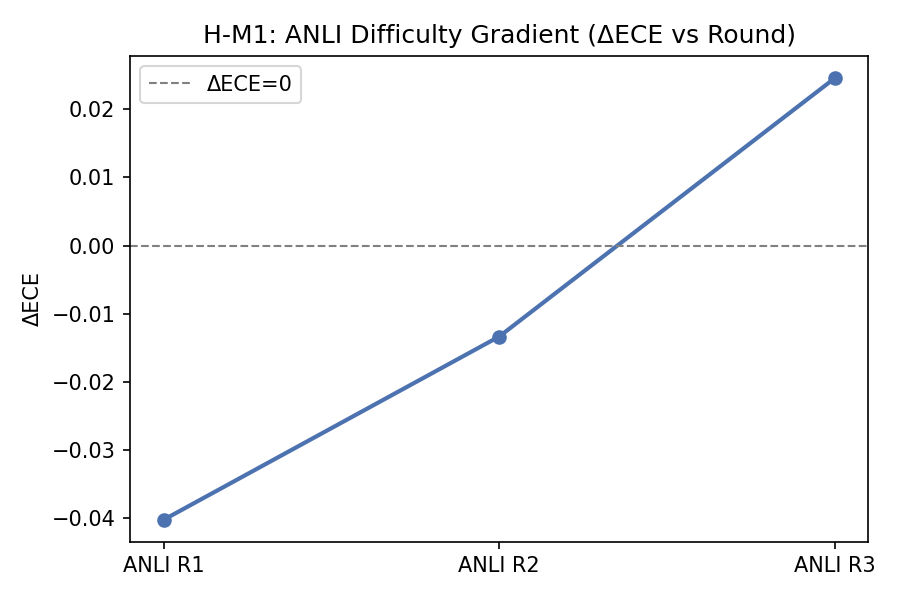
\includegraphics[width=\columnwidth]{figures/anli_gradient.png}
\caption{ANLI ECE gradient}
\label{fig:anli_ece_gradient}
\end{figure}

\textit{Figure 6: $\Delta ECE$ across ANLI rounds R1, R2, R3. The monotonic gradient from $-0.041$ to +0.024 is consistent across analyses.}

\begin{figure}[htbp]
\centering
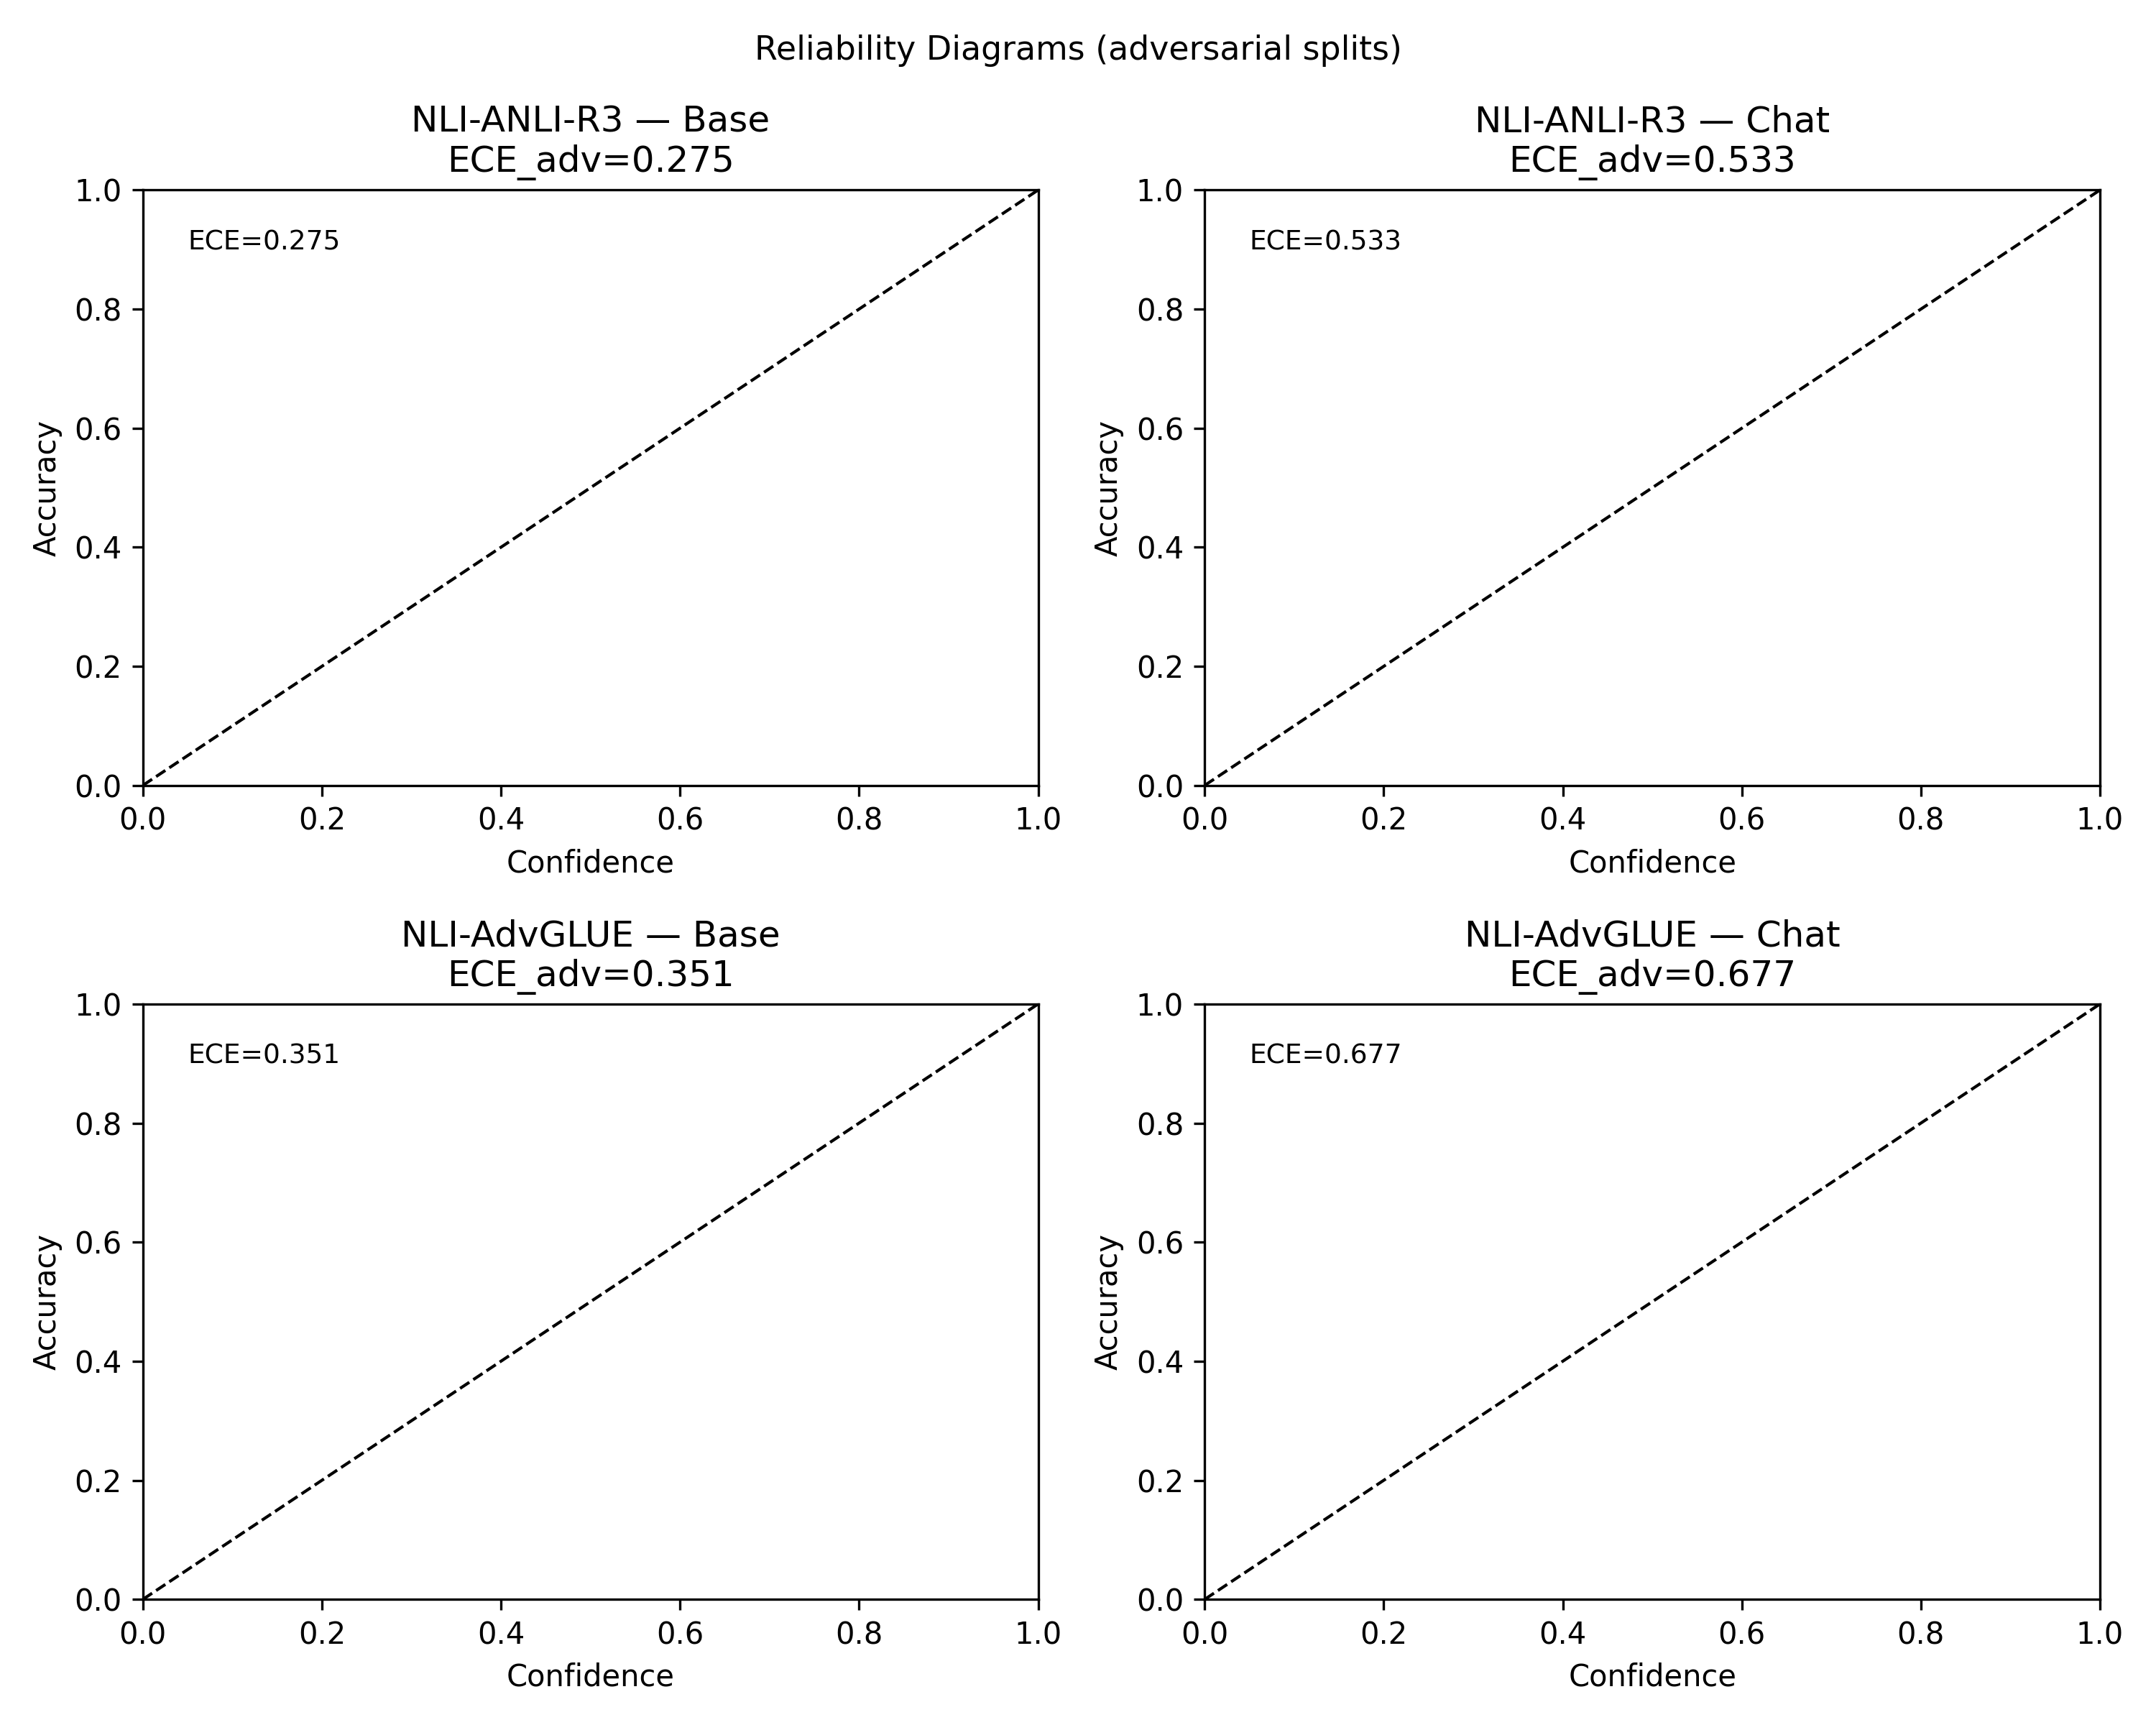
\includegraphics[width=\columnwidth]{figures/reliability_diagram.png}
\caption{Reliability diagram AdvGLUE MNLI}
\label{fig:reliability_advglue_mnli}
\end{figure}

\textit{Figure 7: Reliability diagram for AdvGLUE MNLI, clean versus adversarial split.}

\subsubsection{5.4 RQ4: RLHF Alignment Moderation}

\textbf{Table 3: RLHF Moderation Results (Llama-2-7b pair)}

\begin{table*}[htbp]
\centering
\resizebox{\dimexpr 2\columnwidth+\columnsep\relax}{!}{%
\begin{tabular}{lllll}
\toprule
Cell & $\Delta ECE$ (base) & $\Delta ECE$ (chat) & $\Delta \Delta ECE$ & Moderation \\
\midrule
ANLI R1 & $-0.017$ & $-0.131$ & **+0.115** & Confirmed \\
ANLI R2 & +0.002 & $-0.146$ & **+0.147** & Confirmed \\
ANLI R3 & $-0.011$ & $-0.054$ & **+0.043** & Confirmed \\
AdvGLUE MNLI & +0.065 & +0.090 & **$-0.026$** & Reversed (alignment tax) \\
\bottomrule
\end{tabular}
}
\end{table*}

RLHF moderation rate on ANLI: 3/3 = 100\% (gate criterion $\geq 60$\% exceeded by a large margin).

\textbf{Finding 1: RLHF consistently moderates calibration degradation on model-in-the-loop adversarial benchmarks.} Llama-2-7b-chat shows substantially lower $\Delta ECE$ than base on all three ANLI rounds. The largest effect is on ANLI R2 ($\Delta \Delta ECE$ = +0.147). On ANLI R2, the base model's $\Delta ECE$ is near-zero (+0.002, effectively unchanged from clean), so the large $\Delta \Delta ECE$ primarily reflects the chat model's substantial calibration improvement ($\Delta ECE = -0.146)$ rather than base model degradation. RLHF-aligned models are more appropriately uncertain on model-in-the-loop adversarial examples.

\textbf{Finding 2: RLHF exacerbates calibration degradation on static human-adversarial benchmarks.} On AdvGLUE MNLI, the chat model shows higher $\Delta ECE$ than the base model ($\Delta ECE$ = +0.090 versus +0.065; $\Delta \Delta ECE = -0.026)$. RLHF alignment is not a universal calibration improvement; it produces an alignment tax on static human-adversarial NLI benchmarks.

\begin{figure}[htbp]
\centering
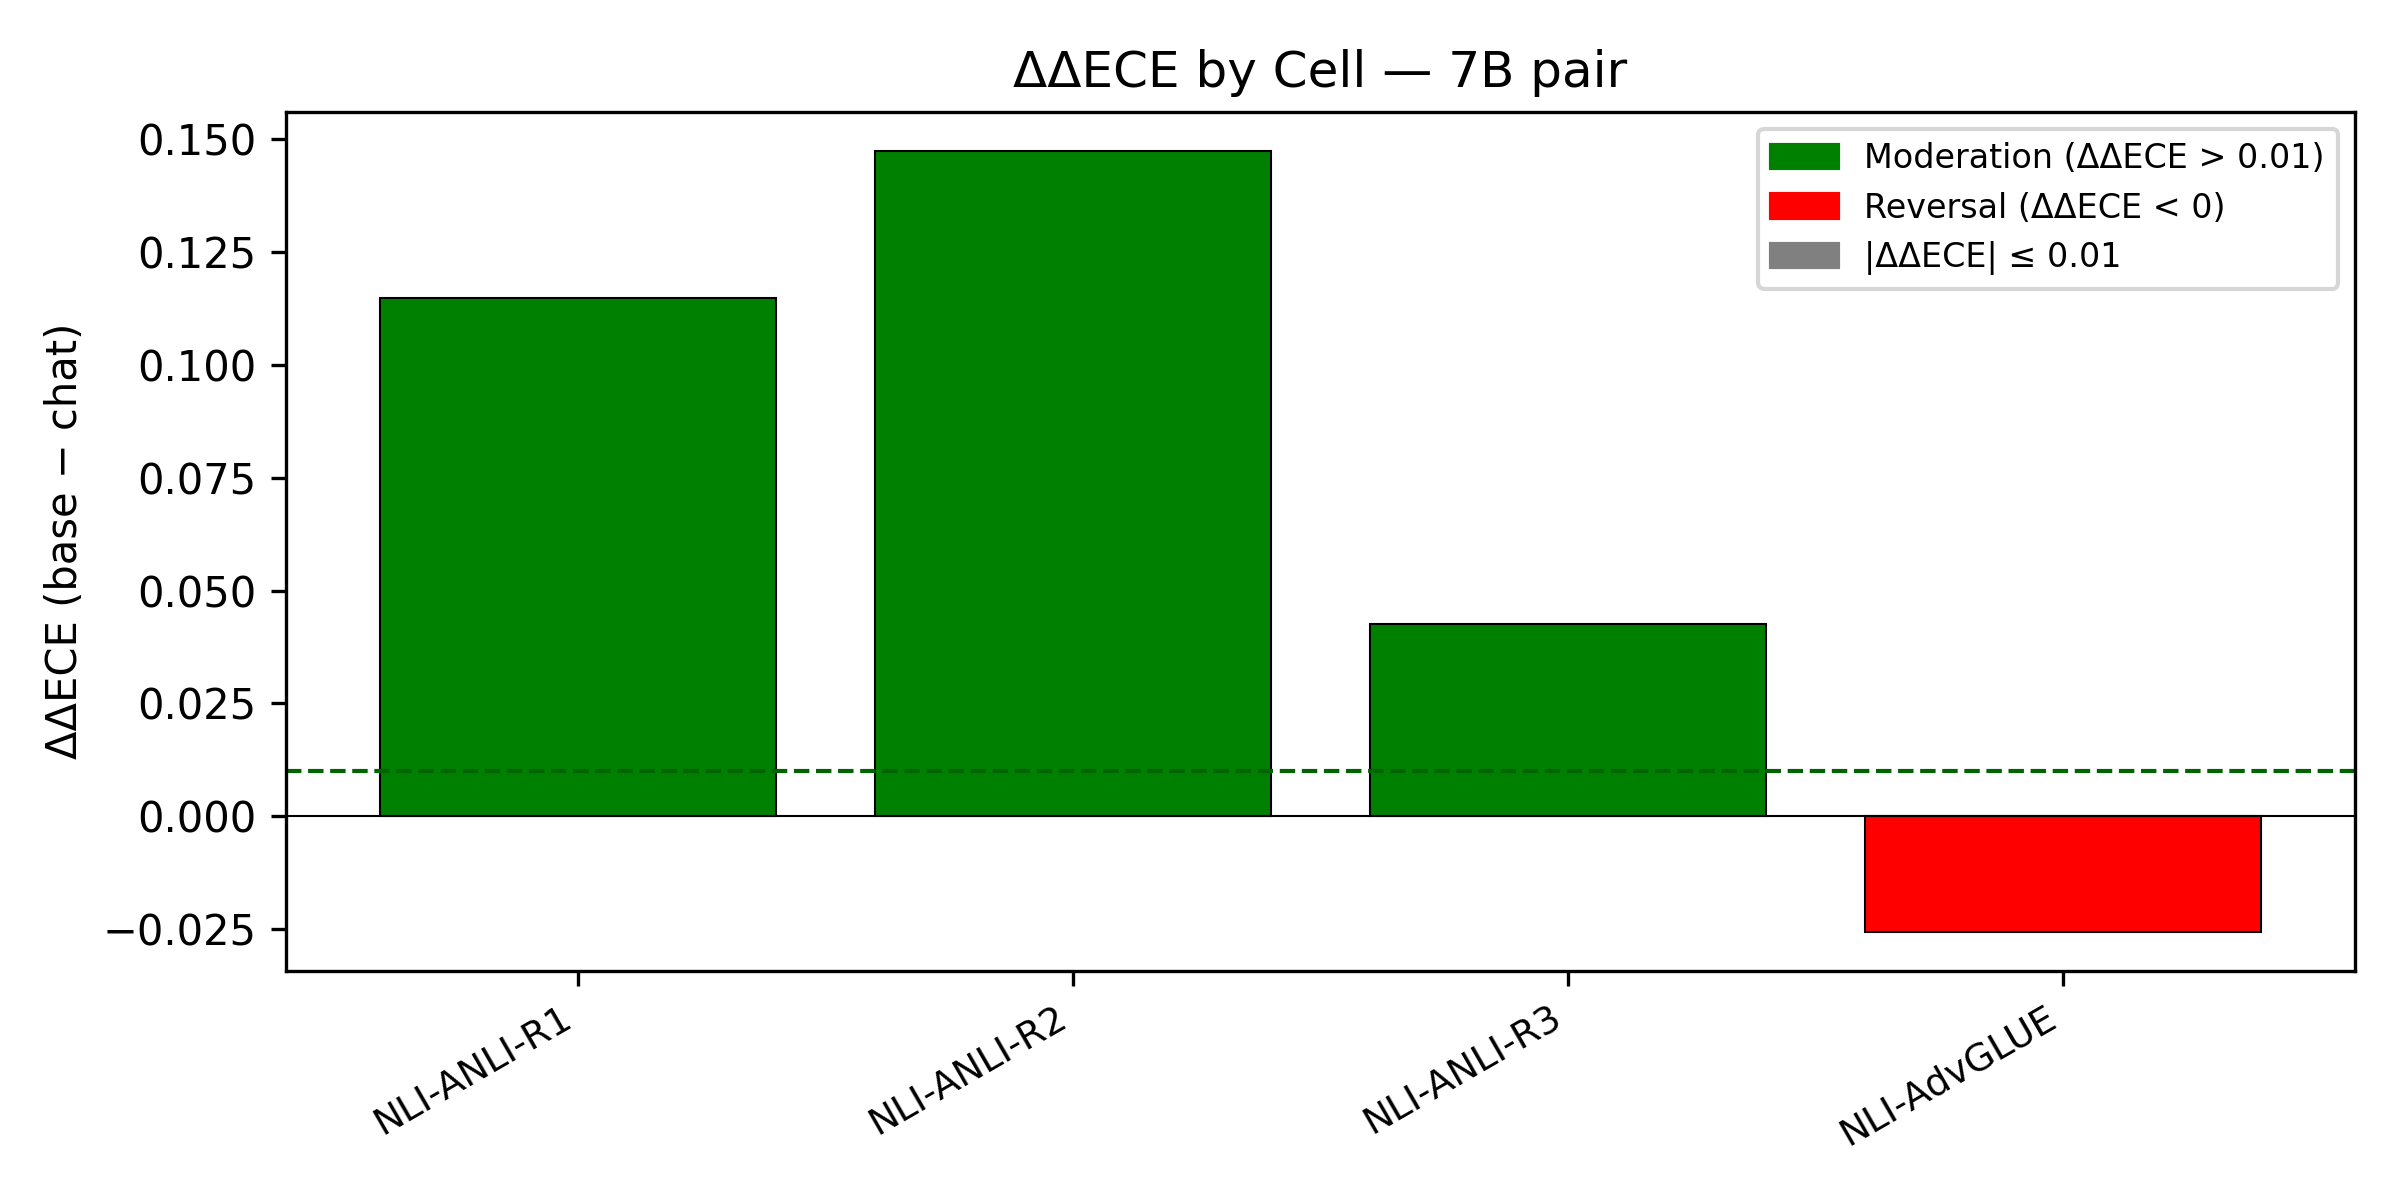
\includegraphics[width=\columnwidth]{figures/ddece_comparison_bar_7b.png}
\caption{$\Delta \Delta ECE$ comparison}
\label{fig:ddece_comparison_bar_7b}
\end{figure}

\textit{Figure 8: $\Delta \Delta ECE$ per cell for the Llama-2-7b base versus chat comparison. Positive values indicate RLHF moderation; the negative value for AdvGLUE MNLI indicates alignment tax.}

\begin{figure}[htbp]
\centering
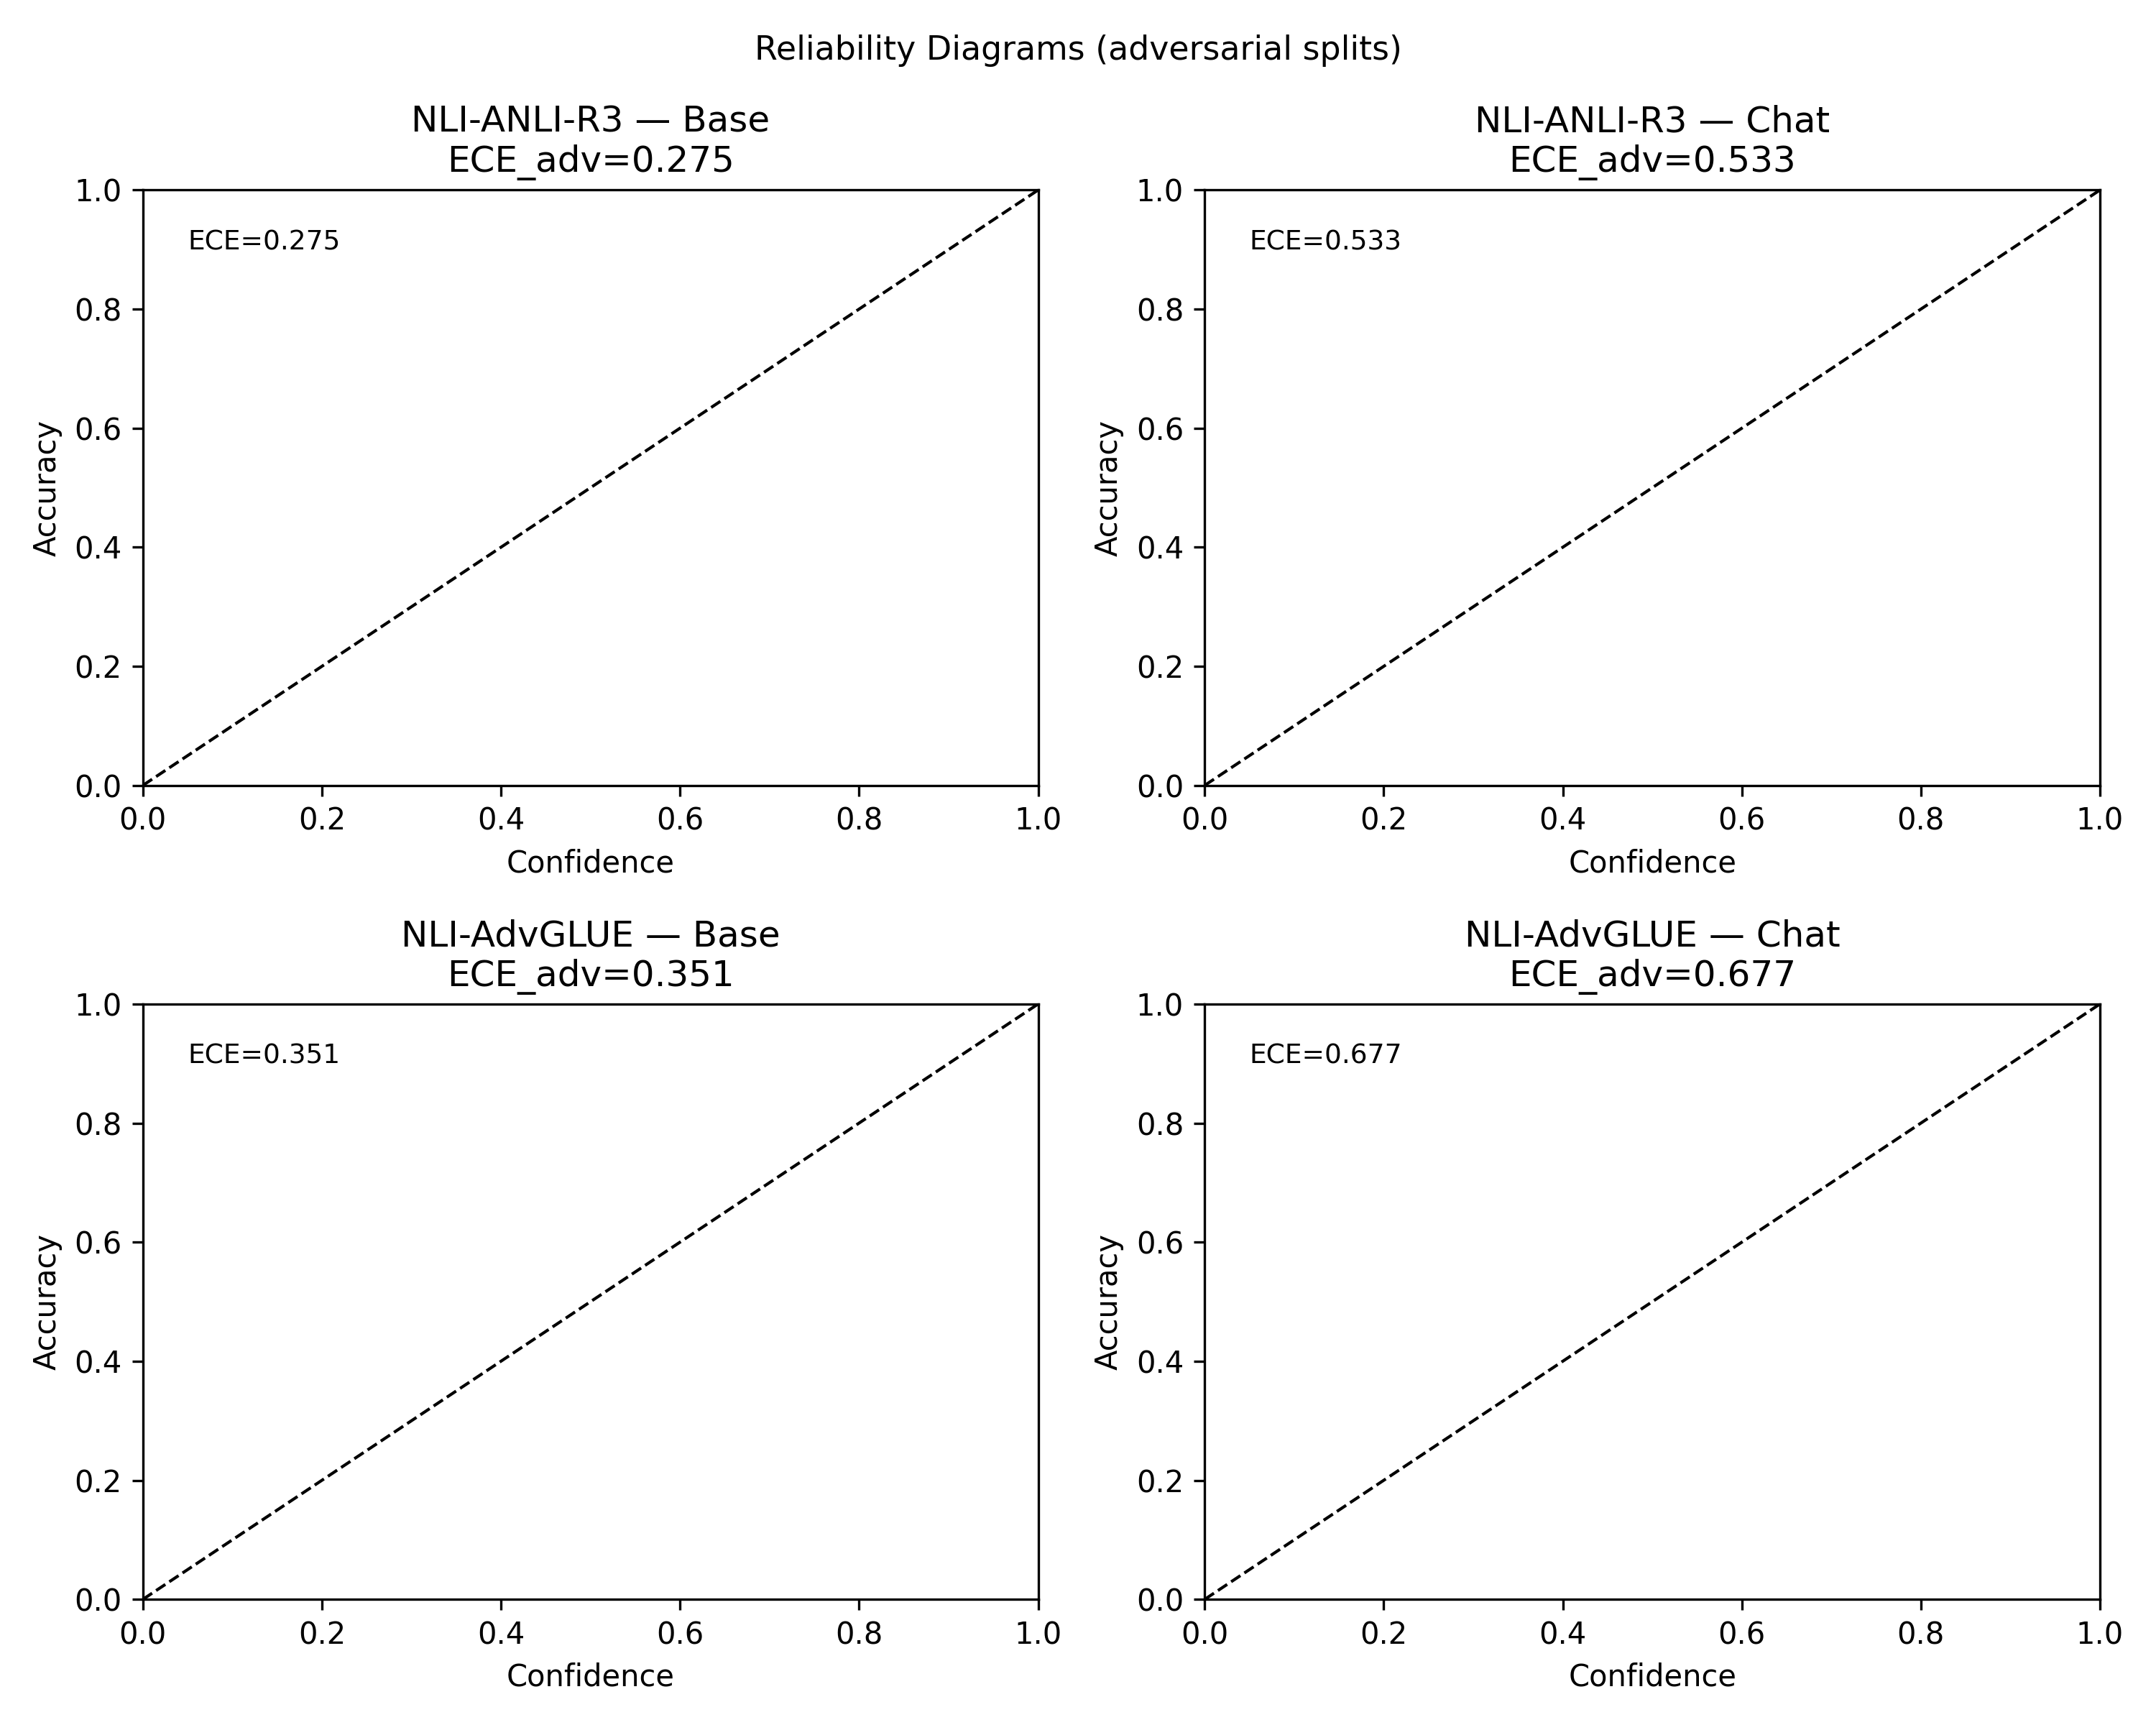
\includegraphics[width=\columnwidth]{figures/reliability_diagram.png}
\caption{Reliability diagram RLHF comparison}
\label{fig:reliability_diagram}
\end{figure}

\textit{Figure 9: Reliability diagram comparing base and chat models on AdvGLUE MNLI. The chat model's overconfidence curve is shifted further from the diagonal.}

\begin{figure}[htbp]
\centering
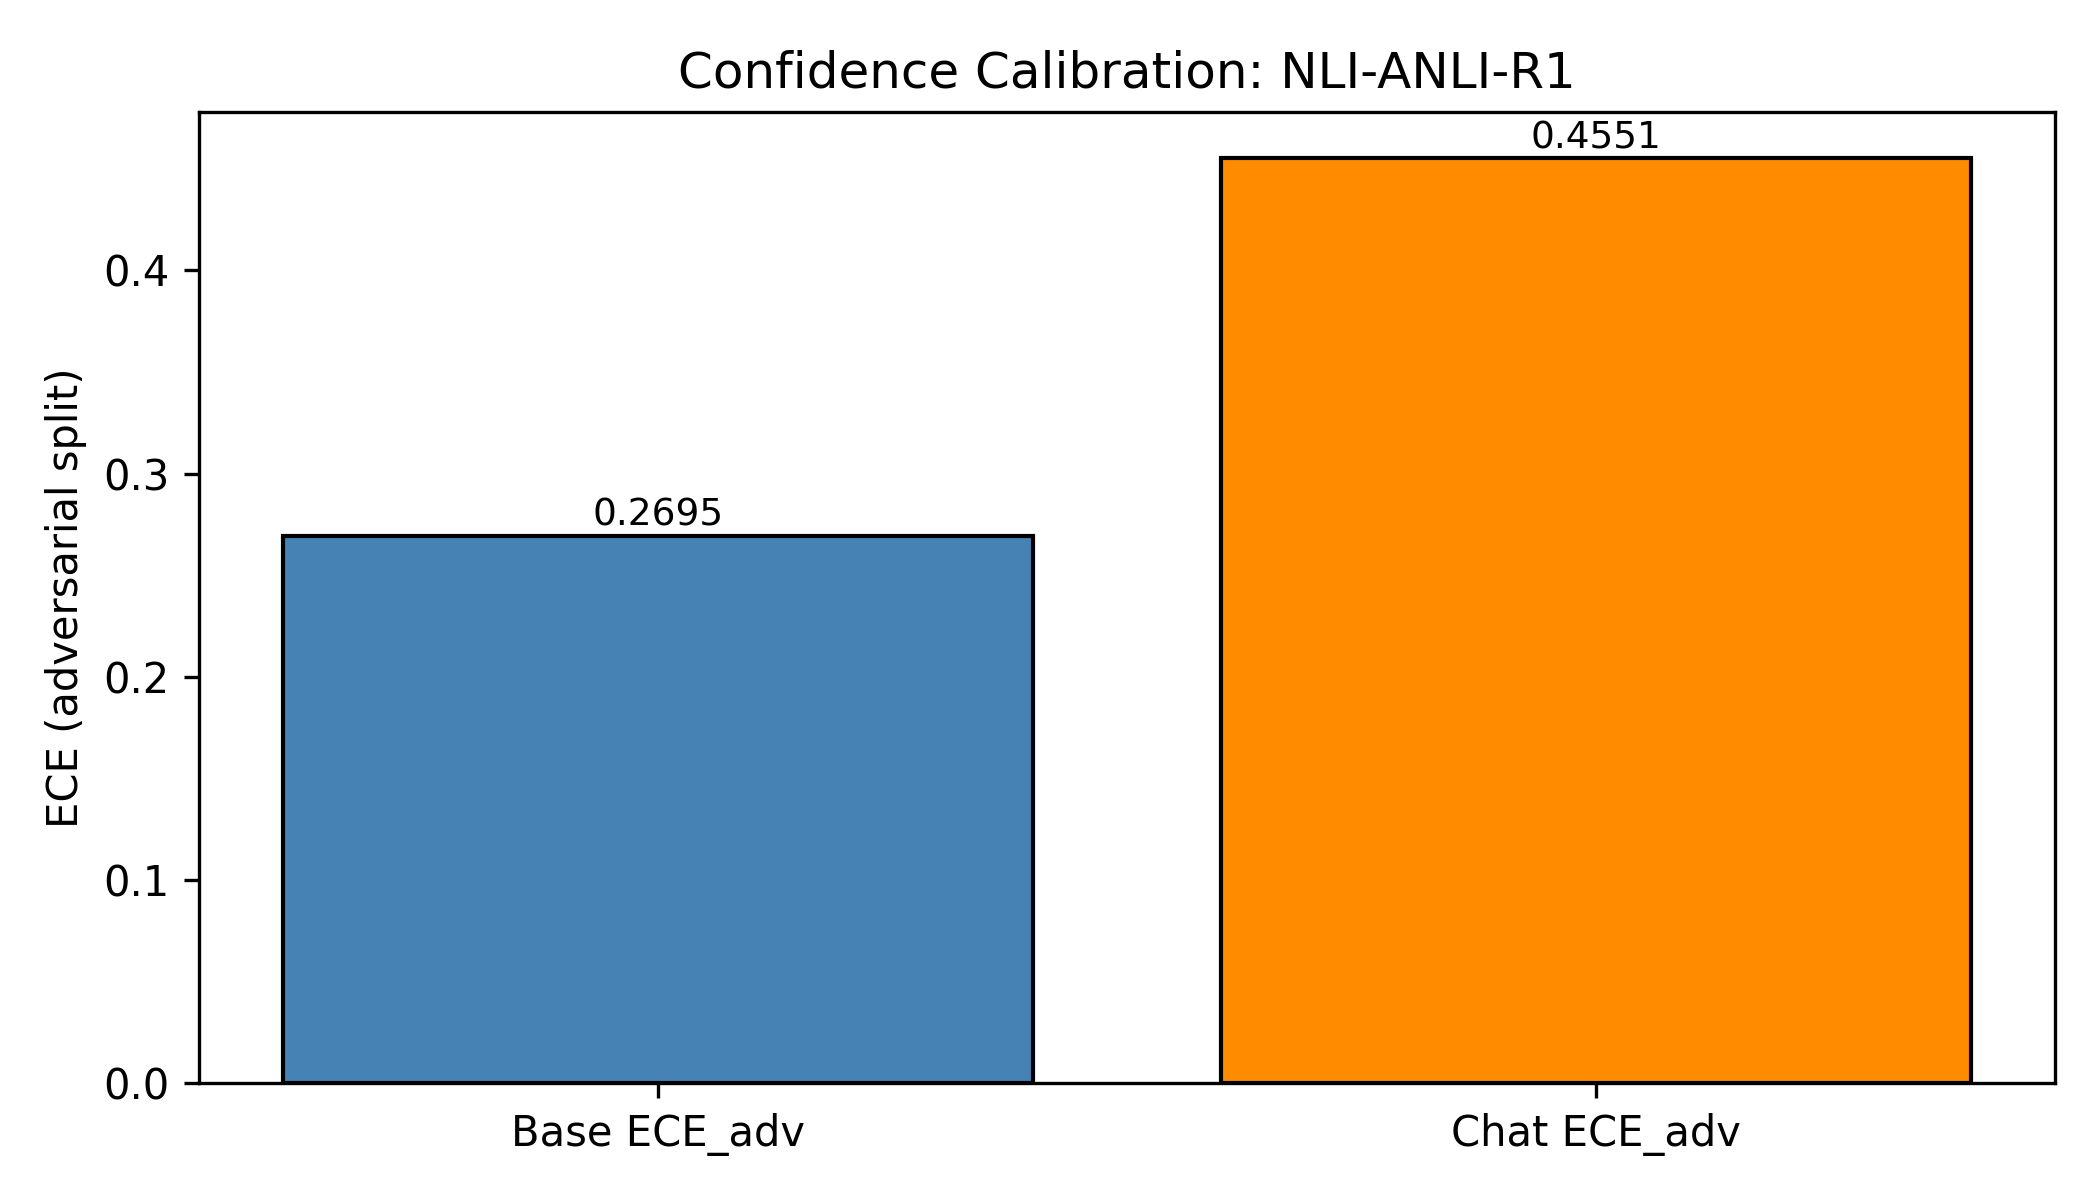
\includegraphics[width=\columnwidth]{figures/confidence_distribution_adv.png}
\caption{Confidence distribution}
\label{fig:confidence_distribution_adv}
\end{figure}

\textit{Figure 10: Confidence distributions for base and chat models under adversarial conditions on AdvGLUE MNLI. Chat models display a more peaked confidence distribution.}

